\section{Часть I. Периодические решения уравнения Мэки-Гласса}

\begin{frame}
	\frametitle{I. Уравнение Мэки--Гласса}
	\begin{equation*}
		\label{eq:MG}
		\dot{v}=-b v+\frac{a \theta^{\gamma} v(t-\tau)}{\theta^{\gamma}+v^{\gamma}(t-\tau)}.
	\end{equation*}
	$a, b, \theta, \tau > 0$, $\gamma \gg 1$, $v(t) > 0$.
\end{frame}

\vspace{2em}

\begin{frame}
	\frametitle{I. Уравнение Мэки--Гласса}
	После перенормировки времени
	\begin{equation*}
		\label{eq:MG_norm}
		\dot{u}=-\beta u + \frac{\alpha u(t - 1)}{1 + u^{\gamma}(t - 1)}.
	\end{equation*}
	
	После экспоненциальной замены:
	\begin{equation}
		\label{eq:MG_x}
		\dot{x}=-\beta+\alpha\frac{e^{x(t-1)-x}}{1 + e^{\gamma x(t-1)}}.
	\end{equation}
	
	$\alpha, \beta > 0$, $\gamma \gg 1$, $u(t) > 0$.
\end{frame}

\begin{frame}
	\frametitle{Релейное уравнение Мэки--Гласса}
	\begin{equation}
		\label{eq:MG_rele}
		\dot{x}=-\beta + \alpha \exp({x(t-1)-x})H(x(t-1)).
	\end{equation}
	%
	\begin{equation}
		\label{eq:H}
		H(x)=\lim\limits_{\gamma\to +\infty}\frac{1}{1 + e^{\gamma x}}=
		\begin{cases}
			0, & x > 0,\\
			\frac{1}{2}, & x = 0,\\
			1, & x < 0.
		\end{cases}
	\end{equation}
	
	\textbf{Теорема} (О решении релейного уравнения).
		Пусть параметры $\alpha,\beta>0$ удовлетворяют условиям
		%
		\begin{equation}
			\label{eq:cond_alpha1}
			\begin{cases}
				\left[
				\begin{array}{ll}
					\alpha > e^{\beta} - e^{-\beta},\\
					\alpha < \beta e^{\beta},
				\end{array}
				\right.\\
				\frac{\alpha}{\beta}e^{\beta}\left(1 + \ln\frac{\beta}{\alpha}\right) < 1,
			\end{cases}
		\end{equation}
%		\begin{equation}
%			\label{eq:cond_alpha2}
%			\alpha > \dfrac{e^{\beta t_1} - 1}{e^{\beta}(t_1 - 1)}.
%		\end{equation}
		%
		Тогда уравнение \eqref{eq:MG_rele} с произвольной непрерывной положительной начальной функцией имеет $T$-периодическое решение
\end{frame}

\begin{frame}
	\frametitle{Решение релейного уравнения Мэки--Гласса}
	\begin{equation*}
	x^*(t)= 
		\begin{cases}
			-\beta t, & t\in[-\sigma_0, 1],\\
			-\beta t +\ln(\alpha e^{\beta}(t - 1)+1), & t\in[1, 2],\\
			-\beta t + \ln(\frac{\alpha^2}{2}e^{2\beta}(t - 2)^2 + \alpha e^{\beta}(t - 1)+1), & t\in[2, t_1],\\
			-\beta t + \ln(\frac{\alpha^2}{2}e^{2\beta}(t_1 - 2)^2 + \alpha e^{\beta}(t_1 - 1)+1), & t\in[t_1, 1 + T].
		\end{cases}
	\end{equation*}
    
    \begin{center}
    	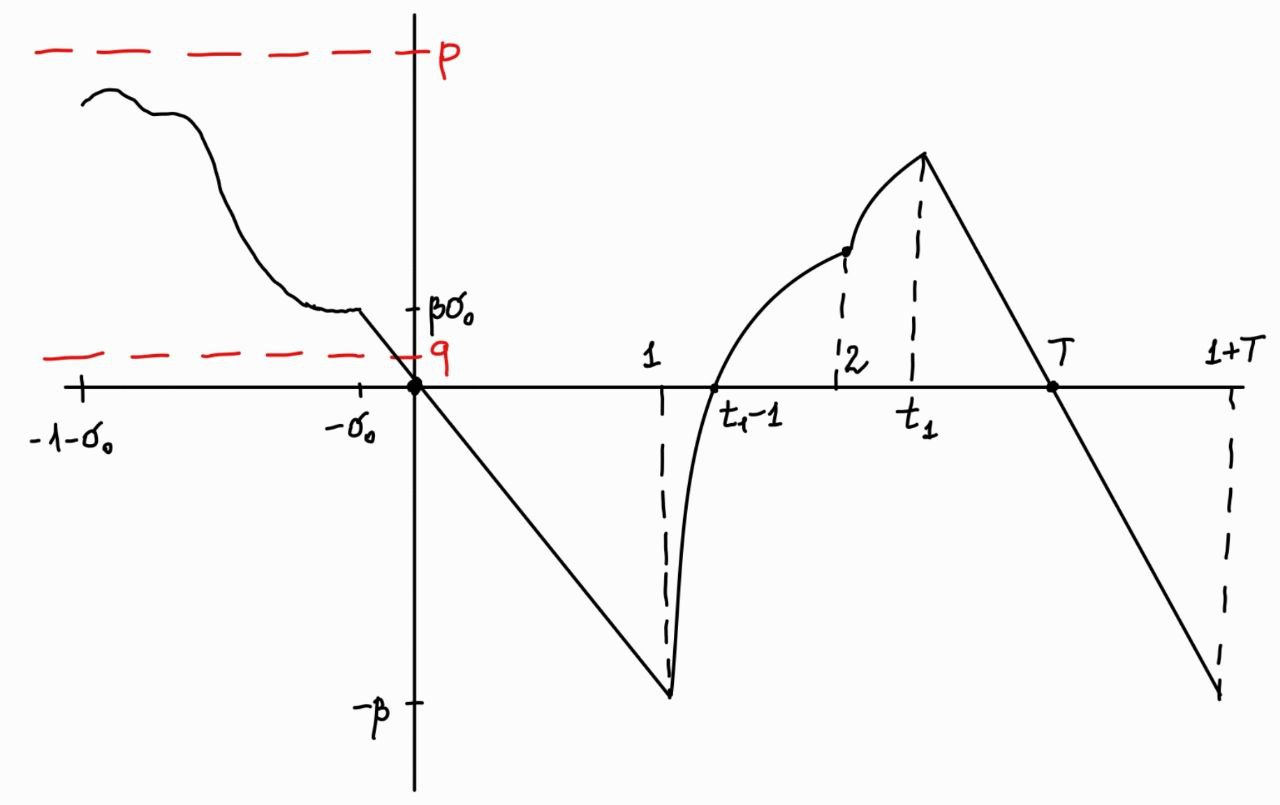
\includegraphics[width=0.8\linewidth]{func1.jpg}
    \end{center}
\end{frame}

\begin{frame}
	\frametitle{Асимптотика решения}
	
	\textbf{Теорема.} Пусть $\delta = \gamma^{-\nu}$, $\nu \in (\frac{1}{2}, 1)$. Уравнение \eqref{eq:MG_x} с произвольной непрерывной положительной функцией $\varphi$ (при некоторых ограничениях на параметры $\alpha, \beta$ имеет решение $x_\gamma^*(t, \varphi)$ с асимптотикой
	\footnotesize
	\begin{equation*}
		\label{eq:sol_x*gamma}
		x^*_\gamma(t, \varphi)= 
		\begin{cases}
			- \beta t + O(\gamma^{-1} e^{-\beta \delta \gamma}), & t\in[-\sigma_0, 1 - \delta],\\
			-\beta + \frac{1}{\gamma} w_0(\tau)|_{\tau=(t - 1)\gamma} + O(\gamma^{-2\nu}), & t \in [1 - \delta,1 + \delta]\\
			- \beta t + \ln(\alpha e^{\beta}(t - 1) + 1) + O(\gamma^{-2\nu}) & t\in[1 + \delta, 2]\\
			- \beta t + \ln(\frac{\alpha^2}{2}e^{2 \beta}(t - 2)^2 + \alpha e^{\beta}(t - 1) + 1) + O(\gamma^{-2\nu}) & t \in [2, t_1 - \delta]\\
			- \beta t_1 + \ln(\eta)+\frac{1}{\gamma} w_1(\tau)|_{\tau=(t - t_1)\gamma} + O(\gamma^{-2\nu}) & t\in[t_1 - \delta, t_1  +\delta]\\
			- \beta t + \ln(\eta) + O(\gamma^{-2\nu}) & t \in [t_1 + \delta, t_2 - \delta]
		\end{cases}
	\end{equation*}
	\normalsize
	где $\eta=\frac{\alpha^2}{2}e^{2\beta}(t_1 - 2)^2 + \alpha e^{\beta}(t_1 - 1) + 1$.
	Асимптотические выражения приведены при $\gamma\to+\infty$.
	Все остатки равномерны по $\varphi$ и $t$ из соответствующих промежутков.
\end{frame}

\begin{frame}
	\frametitle{Основная теорема}
	\textbf{Теорема.} Пусть $S$ --- множество начальных функций,
	\[
	S = \{\varphi \in C[-1 - \sigma_0, -\sigma_0] \, | \, 0 < q \leq \varphi(t) \leq p, \, \varphi(-\sigma_0) = \beta \sigma_0\}.
	\]
	
	Тогда (при некоторых ограничениях на параметры $\alpha, \beta$) для произвольной $\varphi \in S$ и достаточно больших $\gamma$ уравнение \eqref{eq:MG_x} имеет решение $x^*_\gamma(t, \varphi)$ периода $T_{\gamma, \varphi}$, причём
	
	\[
	\lim\limits_{\gamma \to +\infty} \max\limits_{t \in [0, T_{\gamma, \varphi}]} |x^*_\gamma(t, \varphi) - x^*(t)| = 0,
	\]
	
	\[
	\lim\limits_{\gamma \to +\infty} T_{\gamma, \varphi} = T.
	\]
\end{frame}
%
%\begin{frame}
%	\frametitle{Вычисление асимптотики}
%	Пусть
%	$$\delta = \gamma^{-\nu}, \quad \nu \in (1/2, 1).$$
%	%
%	Вне окрестностей точек излома $t_0$ и $t_1$ ищем решение в виде
%	\[
%	x^*_\gamma(t, \varphi) = x^*(t) + \Delta(t, \varphi).
%	\]
%	
%	При $t \in [t_i - \delta, t_i + \delta]$ ищем решение в виде
%	\[
%	x^*_\gamma(t, \varphi) = x^*(t_i) + \frac{1}{\gamma} w_i(\tau)|_{\tau = \gamma(t - t_i)} + \Delta(t, \varphi).
%	\]
%	%
%    \[
%    w_i(\tau) = -\beta \tau - \dfrac{\alpha e^{-x^*(t_i)}}{\dot{x}^*(t_i - 1)} \ln\left(e^{-\dot{x}^*(t_i - 1)\tau} + 1\right) \, \text{при} \, \dot{x}^*(t_i - 1) > 0,
%    \]
%    \[
%    w_i(\tau) = (-\beta + \alpha e^{-x^*(t_i)})\tau - \dfrac{\alpha e^{-x^*(t_i)}}{\dot{x}^*(t_i - 1)} \ln\left(e^{\dot{x}^*(t_i - 1)\tau} + 1\right) \, \text{при} \, \dot{x}^*(t_i - 1) < 0,
%    \]
%\end{frame}

\begin{frame}
	\frametitle{Существование периодического решения}
	
	\begin{center}
		\includegraphics[width=0.8\linewidth]{func2.png}
	\end{center}
\end{frame}

\section{Часть II. Дискретные бегущие волны в полносвязной цепи осцилляторов Мэки--Гласса}


\begin{frame}
	\frametitle{II. Полносвязная цепь осцилляторов Мэки--Гласса}
	
	\begin{equation*}
		\label{eq:system_full_generators}
		\dfrac{d V_{j}}{dt}=- bV_{j} + \dfrac{ac\left(V_{j}(t - \tau) + \sum\limits_{k = 0, k\neq j}^{m}V_{k}(t)\right)}{1 + \left(c\left(V_{j}(t - \tau) + \sum\limits_{k = 0, k\neq j}^{m}V_{k}(t)\right)\right)^{\gamma}}, \quad j=0,1,\ldots,m.
	\end{equation*}
	
	$a, b, c, \tau > 0$, $\gamma \gg 0$
\end{frame}

\begin{frame}
	\frametitle{II. Полносвязная цепь осцилляторов Мэки--Гласса}
	
	После перенормировок и предельного перехода при $\gamma \to +\infty$:
	
	\begin{equation*}
		\dot{u}_j=-\beta u_j+\alpha\left(u_j(t-1)+ \sum\limits_{k=0, k\neq j}^{m} u_{k}(t)\right)F\left(u_j(t-1)+\sum\limits_{k=0, k\neq j}^{m} u_{k}(t)\right).
	\end{equation*}

%	\begin{equation}
%		\label{eq:mg_relay_w}
%		\dot{u}=-\beta u+\alpha w(t) F(w(t)), \text{ где }
%	\end{equation}
%	%
%	\begin{equation*}
%	w(t) = \sum\limits_{s = 0}^m u(t - \tau_s).
%	\end{equation*}
\end{frame}


\begin{frame}
	\frametitle{Дискретная бегущая волна}
	
	\begin{equation}
		\label{eq:discrete_wave}
		u_j(t) = u(t + k_j\Delta),   
	\end{equation}
	где $\{k_0, k_1, \ldots, k_m\}$ --- перестановка номеров $\{0, 1, \ldots, m\}$, $u(t)$ --- некоторая $T-$периодическая функция, $\Delta > 0$ --- сдвиг.
	
	\small
	\begin{equation}
		\label{eq:mg_relay_0}
		\dot{u} = -\beta u+\alpha\left(u(t-1)+ \sum_{s=0,s\neq j}^{m}u(t+(k_s-k_j)\Delta)\right)F\left(\dots\right).
	\end{equation}
	\normalsize
	
	Если $u(t + (m + 1)\Delta) = u(t)$, т.е. 
	\[(m + 1)\Delta = pT \text{ для некоторого } p \in \mathbf{N},\]
	
	все уравнения системы обращаются в
	
	\small
	\begin{equation}
		\label{eq:mg_relay_0}
		\dot{u} = -\beta u+\alpha\left(u(t - 1) + \sum_{s=1}^{m}u(t + s\Delta)\right)F\left(\dots\right).
	\end{equation}
	\normalsize
	
	
\end{frame}

\begin{frame}
	\frametitle{Решение вспомогательного уравнения}
	\small
	\begin{equation*}
		\label{eq:u_star}
		u_*(t)=
		\begin{cases}
			u_0 e^{-\beta t}(\alpha A(t-t_0)+1) & \text{ при } t\in[t_0,t_0+1].
			\\
			u_0 e^{-\beta t}\left(\frac{\alpha^2}{2}Ae^{\beta}(t-t_0-1)^2+\alpha A(t-t_0)+1\right) & \text{ при } t\in[t_0+1,t_1],
			\\
			u_0 e^{-\beta t}\left(\frac{\alpha^2}{2}Ae^{\beta}(t_1-t_0-1)^2+\alpha A(t_1-t_0)+1\right) & \text{ при } t\in[t_1,t_0+T],
		\end{cases}
	\end{equation*}
	\normalsize
	%
	\[
	u_*(t+T)\equiv u_*(t),
	\]
	%
	\begin{equation*}
		\label{eq:mg_period_T}
		T = \dfrac{1}{\beta}\ln\left( \frac{\alpha^2}{2}Ae^{\beta}(t_1-t_0-1)^2+\alpha A(t_1-t_0)+1\right). 
	\end{equation*}
	
	Здесь $A = e + e^{\Delta} + e^{2\Delta} + \ldots + e^{m\Delta}$, $t_0$, $t_1$ --- точки переключения.
	
	\begin{center}
		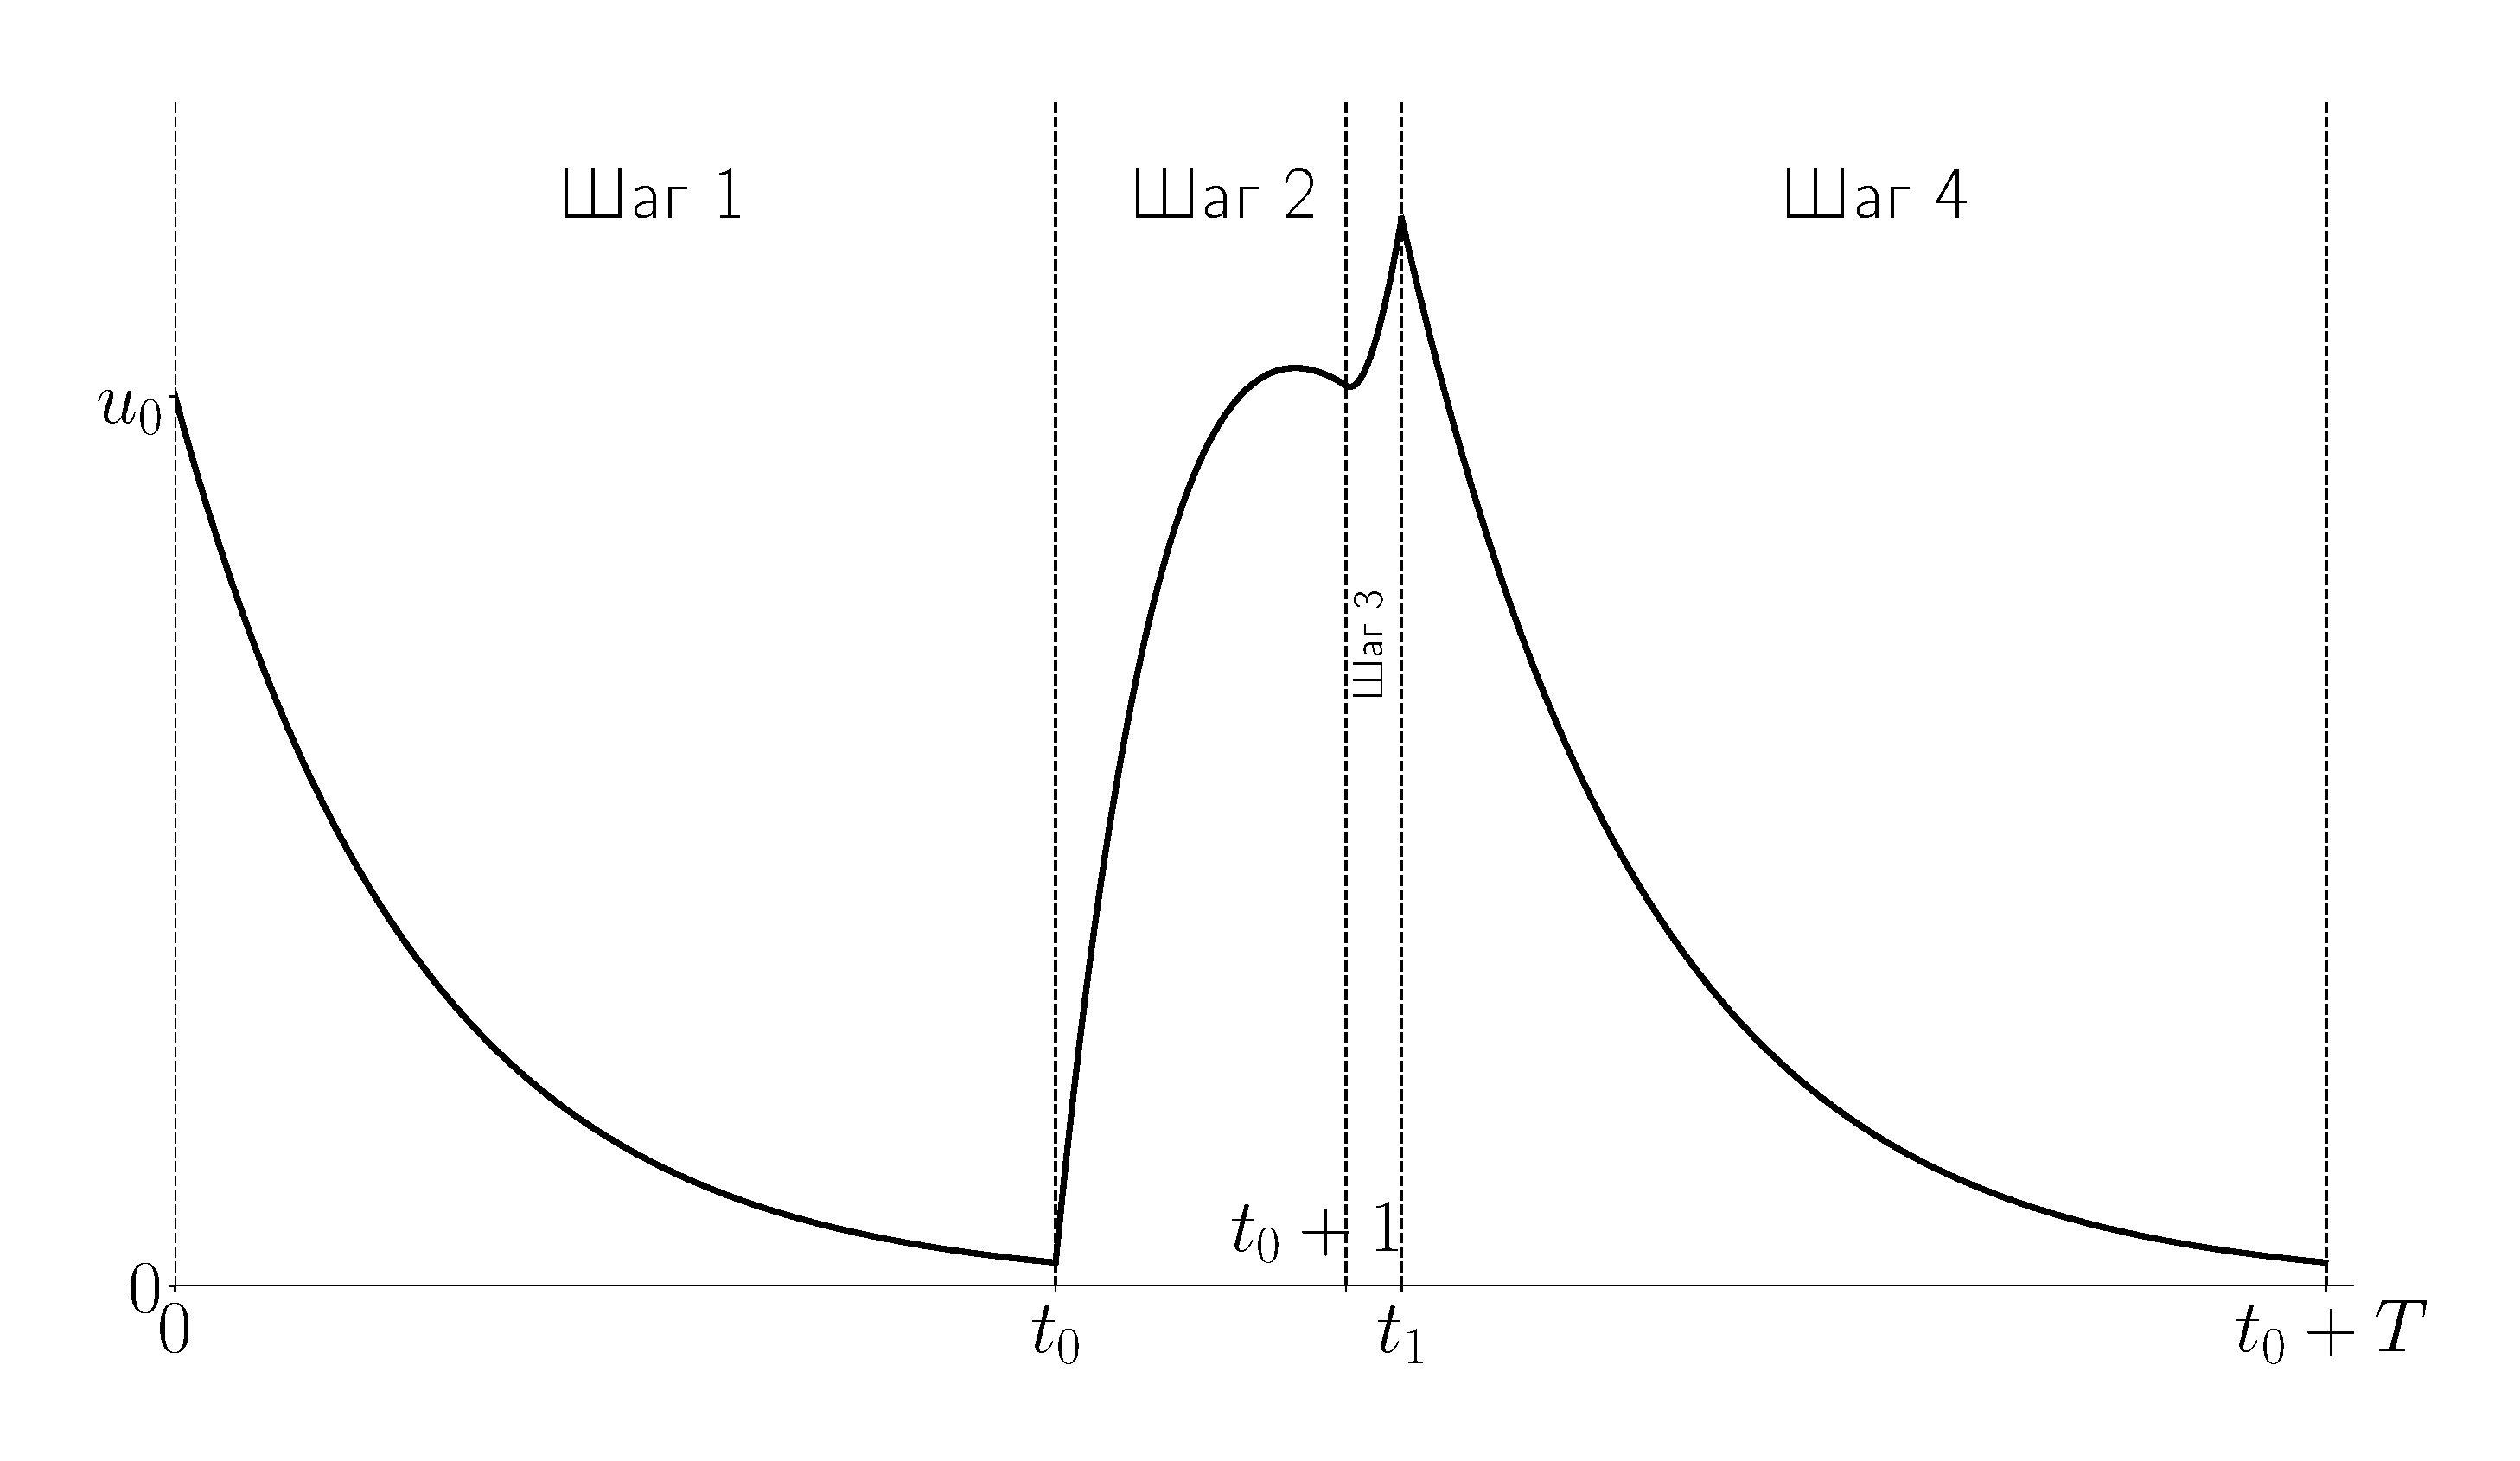
\includegraphics[width=0.6\textwidth]{u_star.eps}
	
	\end{center}
\end{frame}

\begin{frame}
	\frametitle{Бегущая волна: теорема существования}
	
	\textbf{Теорема.} 
	Для произвольных $\beta > 0$, $\alpha \geqslant e^{\beta\left(1 + \frac{1}{e^{\beta}}\right)} - 1$ найдётся $\Delta > 1$, при котором вспомогательное уравнение с параметрами $\alpha, \beta, \Delta$ имеет $T$-периодическое решение, причём $T = (m + 1) \Delta$. Соответствующий набор функций $u_j(t) = u(t + j \Delta), j = 0, \ldots m$ (с точностью до нумерации компонент) является решением в виде дискретной бегущей волны.
\end{frame}

\begin{frame}
	\frametitle{Бегущая волна: численные результаты}
	
	\begin{center}
		\includegraphics[width=0.9\linewidth]{a5p0_b1p2_m2_solution_start.eps}
		
		\includegraphics[width=0.9\linewidth]{a5p0_b1p2_m2_const_start.eps}
		
		\includegraphics[width=0.9\linewidth]{a5p0_b1p2_m2_random_start.eps}
	\end{center}
\end{frame}

\section{Часть III. Режимы двухкластерной синхронизации в полносвязной цепи осцилляторов Мэки-Гласса}

\begin{frame}
	\frametitle{Двухластерная синхронизация в полносвязной системе}
	
	\begin{center}
		\includegraphics[width=0.4\textwidth]{full_mesh.png}
	\end{center}
	
	\vspace{20px}
	
	$$\dot{u}_i(t) = -\beta u_i(t) + \alpha \Phi\big(u_i(t - 1) + \delta\sum\limits_{j \neq i} u_j(t)\big).$$
\end{frame}

\begin{frame}
	\frametitle{Двухкластерная синхронизация в полносвязной системе}
	
	\begin{wrapfigure}{r}{0.5\textwidth}
		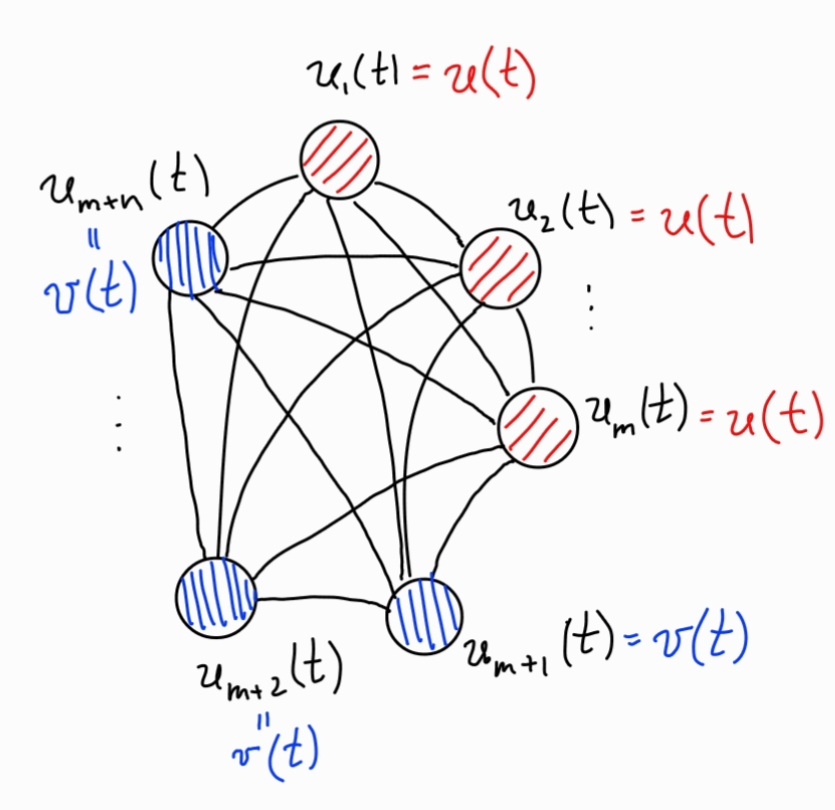
\includegraphics[width=\linewidth]{cluster.jpg}
	\end{wrapfigure}
	
	Ищем периодическое решение
	
	$$u_1(t) \equiv \dots \equiv u_m(t) \equiv u(t)$$
	$$u_{m + 1}(t) \equiv \dots \equiv u_{m + n}(t) \equiv v(t).$$
	
\end{frame}

\begin{frame}
	\frametitle{Двухластерная синхронизация в полносвязной системе}
	
	\begin{equation*}
		\begin{cases}
			\dot{u} = -\beta u + \alpha \, \Phi \big(u(t - 1) + \delta (m - 1) u + \delta n v\big),\\
			\dot{v} = -\beta v + \alpha  \, \Phi \big(v(t - 1) + \delta m u + \delta (n - 1) v\big).
		\end{cases},
	\end{equation*}
	
	где 
	\begin{equation*}
		\Phi(x) = \dfrac{x}{1 + x^\gamma}.
	\end{equation*}
\end{frame}

\begin{frame}
	\frametitle{Двухкластерная синхронизация в полносвязной системе}
	Произведём замены 
	\begin{equation}
		\label{eq:tilde_change}
		\begin{cases}
			\tilde{u}(t) = u(t - 1) + \delta (m - 1) u + \delta n v,\\ \tilde{v}(t) = v(t - 1) + \delta m u + \delta (n - 1) v.
		\end{cases}
	\end{equation}
	
	\bigskip
	
	\textbf{Теорема 1.} Пусть $\tilde{u}, \tilde{v}$ --- неотрицательные $T$-периодические непрерывно дифференцируемые функции. Тогда при $\delta > 1$ существуют и определены единственным образом неотрицательные $T$-периодические непрерывно дифференцируемые функции $u, v$, удовлетворяющие системе \eqref{eq:tilde_change}.
\end{frame}


\begin{frame}
	\frametitle{Двухластерная синхронизация в полносвязной системе}
	
	Система примет вид
	
	\begin{equation}
		\label{eq:mg_cluster_system_tilde}
		\begin{cases}
			\dot{\tilde{u}} = -\beta \tilde{u} + \alpha \big(F(\tilde{u}(t - 1)) + \delta (m - 1) \, F(\tilde{u}) + \delta n \, F(\tilde{v})\big),\\
			\dot{\tilde{v}} = -\beta \tilde{v} + \alpha \big(F(\tilde{v}(t - 1)) + \delta m \, F(\tilde{u}) + \delta (n - 1) \, F(\tilde{v})\big).
		\end{cases}
	\end{equation}
	
	\bigskip
	
	\textbf{Теорема 2.} Если неотрицательные $T$-периодические функции $\tilde{u}, \tilde{v}$ являются решением системы \eqref{eq:mg_cluster_system_tilde}, то выраженные из соотношений \eqref{eq:tilde_change} функции $u, v$ являются решением системы
	
	\begin{equation*}
		\begin{cases}
			\dot{u} = -\beta u + \alpha \, F \bigg(u(t - 1) + \delta (m - 1) u + \delta n v\bigg),\\
			\dot{v} = -\beta v + \alpha  \, F \bigg(v(t - 1) + \delta m u + \delta (n - 1) v\bigg).
		\end{cases}
	\end{equation*}
\end{frame}

\begin{frame}{Экспоненциальная замена}
	
	После экспоненциальной замены
	\begin{equation}
		\label{eq:exp_change}
		\tilde{u} = e^x, \quad \tilde{v} = e^y
	\end{equation}
	и ввода функции $$G(x) = e^{-x} \, F (e^x) = \dfrac{1}{1 + e^{\gamma x}},$$ получаем итоговый вид системы:
	\footnotesize
	\begin{equation*}
		\label{eq:system_main}
		\begin{cases}
			\dot{x} = -\beta + \alpha \left(e^{x(t - 1) - x} G(x(t - 1)) + \delta (m - 1) G(x) + \delta n e^{y - x} G(y)\right),\\
			\dot{y} = -\beta + \alpha \left(e^{y(t - 1) - y} G(y(t - 1)) + \delta m e^{x - y} G(x) + \delta (n - 1) G(y)\right).
		\end{cases}
	\end{equation*}
	\normalsize
\end{frame}

\begin{frame}{Переход к релейной системе}
	Пусть 
	\begin{equation*}
		\tilde{G}(x) = \lim\limits_{\gamma \to +\infty} G(x) = \lim\limits_{\gamma \to +\infty} \dfrac{1}{1 + e^{\gamma x}} = \begin{cases}
			1, & x > 0;\\
			1/2, & x = 0;\\
			0, & x < 0.
		\end{cases}
	\end{equation*}
	
	Перейдём к \emph{релейной} системе
	\footnotesize
	\begin{equation*}
		\label{eq:system_main}
		\begin{cases}
			\dot{x} = -\beta + \alpha \left(e^{x(t - 1) - x} \tilde{G}(x(t - 1)) + \delta (m - 1) \tilde{G}(x) + \delta n e^{y - x} \tilde{G}(y)\right),\\
			\dot{y} = -\beta + \alpha \left(e^{y(t - 1) - y} \tilde{G}(y(t - 1)) + \delta m e^{x - y} \tilde{G}(x) + \delta (n - 1) \tilde{G}(y)\right).
		\end{cases}
	\end{equation*}
	\normalsize
	
	\pause
	\bigskip
	
	Множество начальных функций:
	\begin{multline*}
		\label{eq:initial_set}
		S = \{\varphi, \psi \in C[-1, 0] \,|\, \varphi(t) > 0, \psi(t) > 0, \\ x_0 = \varphi(0), y_0 = \psi(0), x_0 > y_0 \}.
	\end{multline*}
\end{frame}


\begin{frame}{Первый шаг решения системы}
	
	Пусть $\alpha > \dfrac{\beta}{\delta (n - 1)}$. Как продолжить решение?
	
	\begin{center}
		\includegraphics[width=0.7\textwidth]{1_step.png}
	\end{center}
	
	\pause
	
	\bigskip
	
	Решение продолжается только вдоль прямой $y = 0$. Тогда $G(0) = \dfrac{\beta}{\delta(n - 1)} = \dfrac{1}{2}$?
	
\end{frame}


\begin{frame}{Обобщённое решение уравнения}
	Введём функции $g_x(x, t)$, $g_y(y, t)$; перепишем систему в виде:
	\footnotesize
	\begin{equation*}
		\label{eq:generalized_system}
		\begin{cases}
			\dot{x} = -\beta + \alpha \left(e^{x(t - 1) - x} g_x(x(t - 1), t - 1) + \delta (m - 1) g_x(x, t) + \delta n e^{y - x} g_y(y, t)\right),\\
			\dot{y} = -\beta + \alpha \left(e^{y(t - 1) - y} g_y(y(t - 1), t - 1) + \delta m e^{x - y} g_x(x, t) + \delta (n - 1) g_y(y, t)\right),\\
			g_x(x, t) = \tilde{G}(x) \text{  при  } x \neq 0,\\
			g_y(y, t) = \tilde{G}(y) \text{  при  } y \neq 0. 
		\end{cases}
	\end{equation*}
	\normalsize
	
	\pause
	
	\bigskip
	
	Решение данной системы называется обобщённым решением релейной системы.
	
\end{frame}

\begin{frame}{Решение системы}
	\textbf{Теорема 3.} При ограничениях на параметры
	\footnotesize
	\begin{equation*}
		\label{eq:constraint_2}
		\beta < \alpha \delta (m - 1), \quad \beta < \alpha \delta (n - 1),
	\end{equation*}
	\begin{equation*}
		\label{eq:constraint_3}
		e^{\beta} \cdot \dfrac{n - \delta(n - 1)}{\delta (n - 1)^2} > \dfrac{1}{n - 1} + \dfrac{1}{\delta(m - 1)}, \quad
		e^{\beta} \cdot \dfrac{m - \delta(m - 1)}{\delta (m - 1)^2} > \dfrac{1}{\delta(n - 1)} + \dfrac{1}{m - 1}.
	\end{equation*}
	\normalsize
	
	релейная система с начальной функцией из множества $S$ имеет единственное (обобщённое) решение следующего вида
	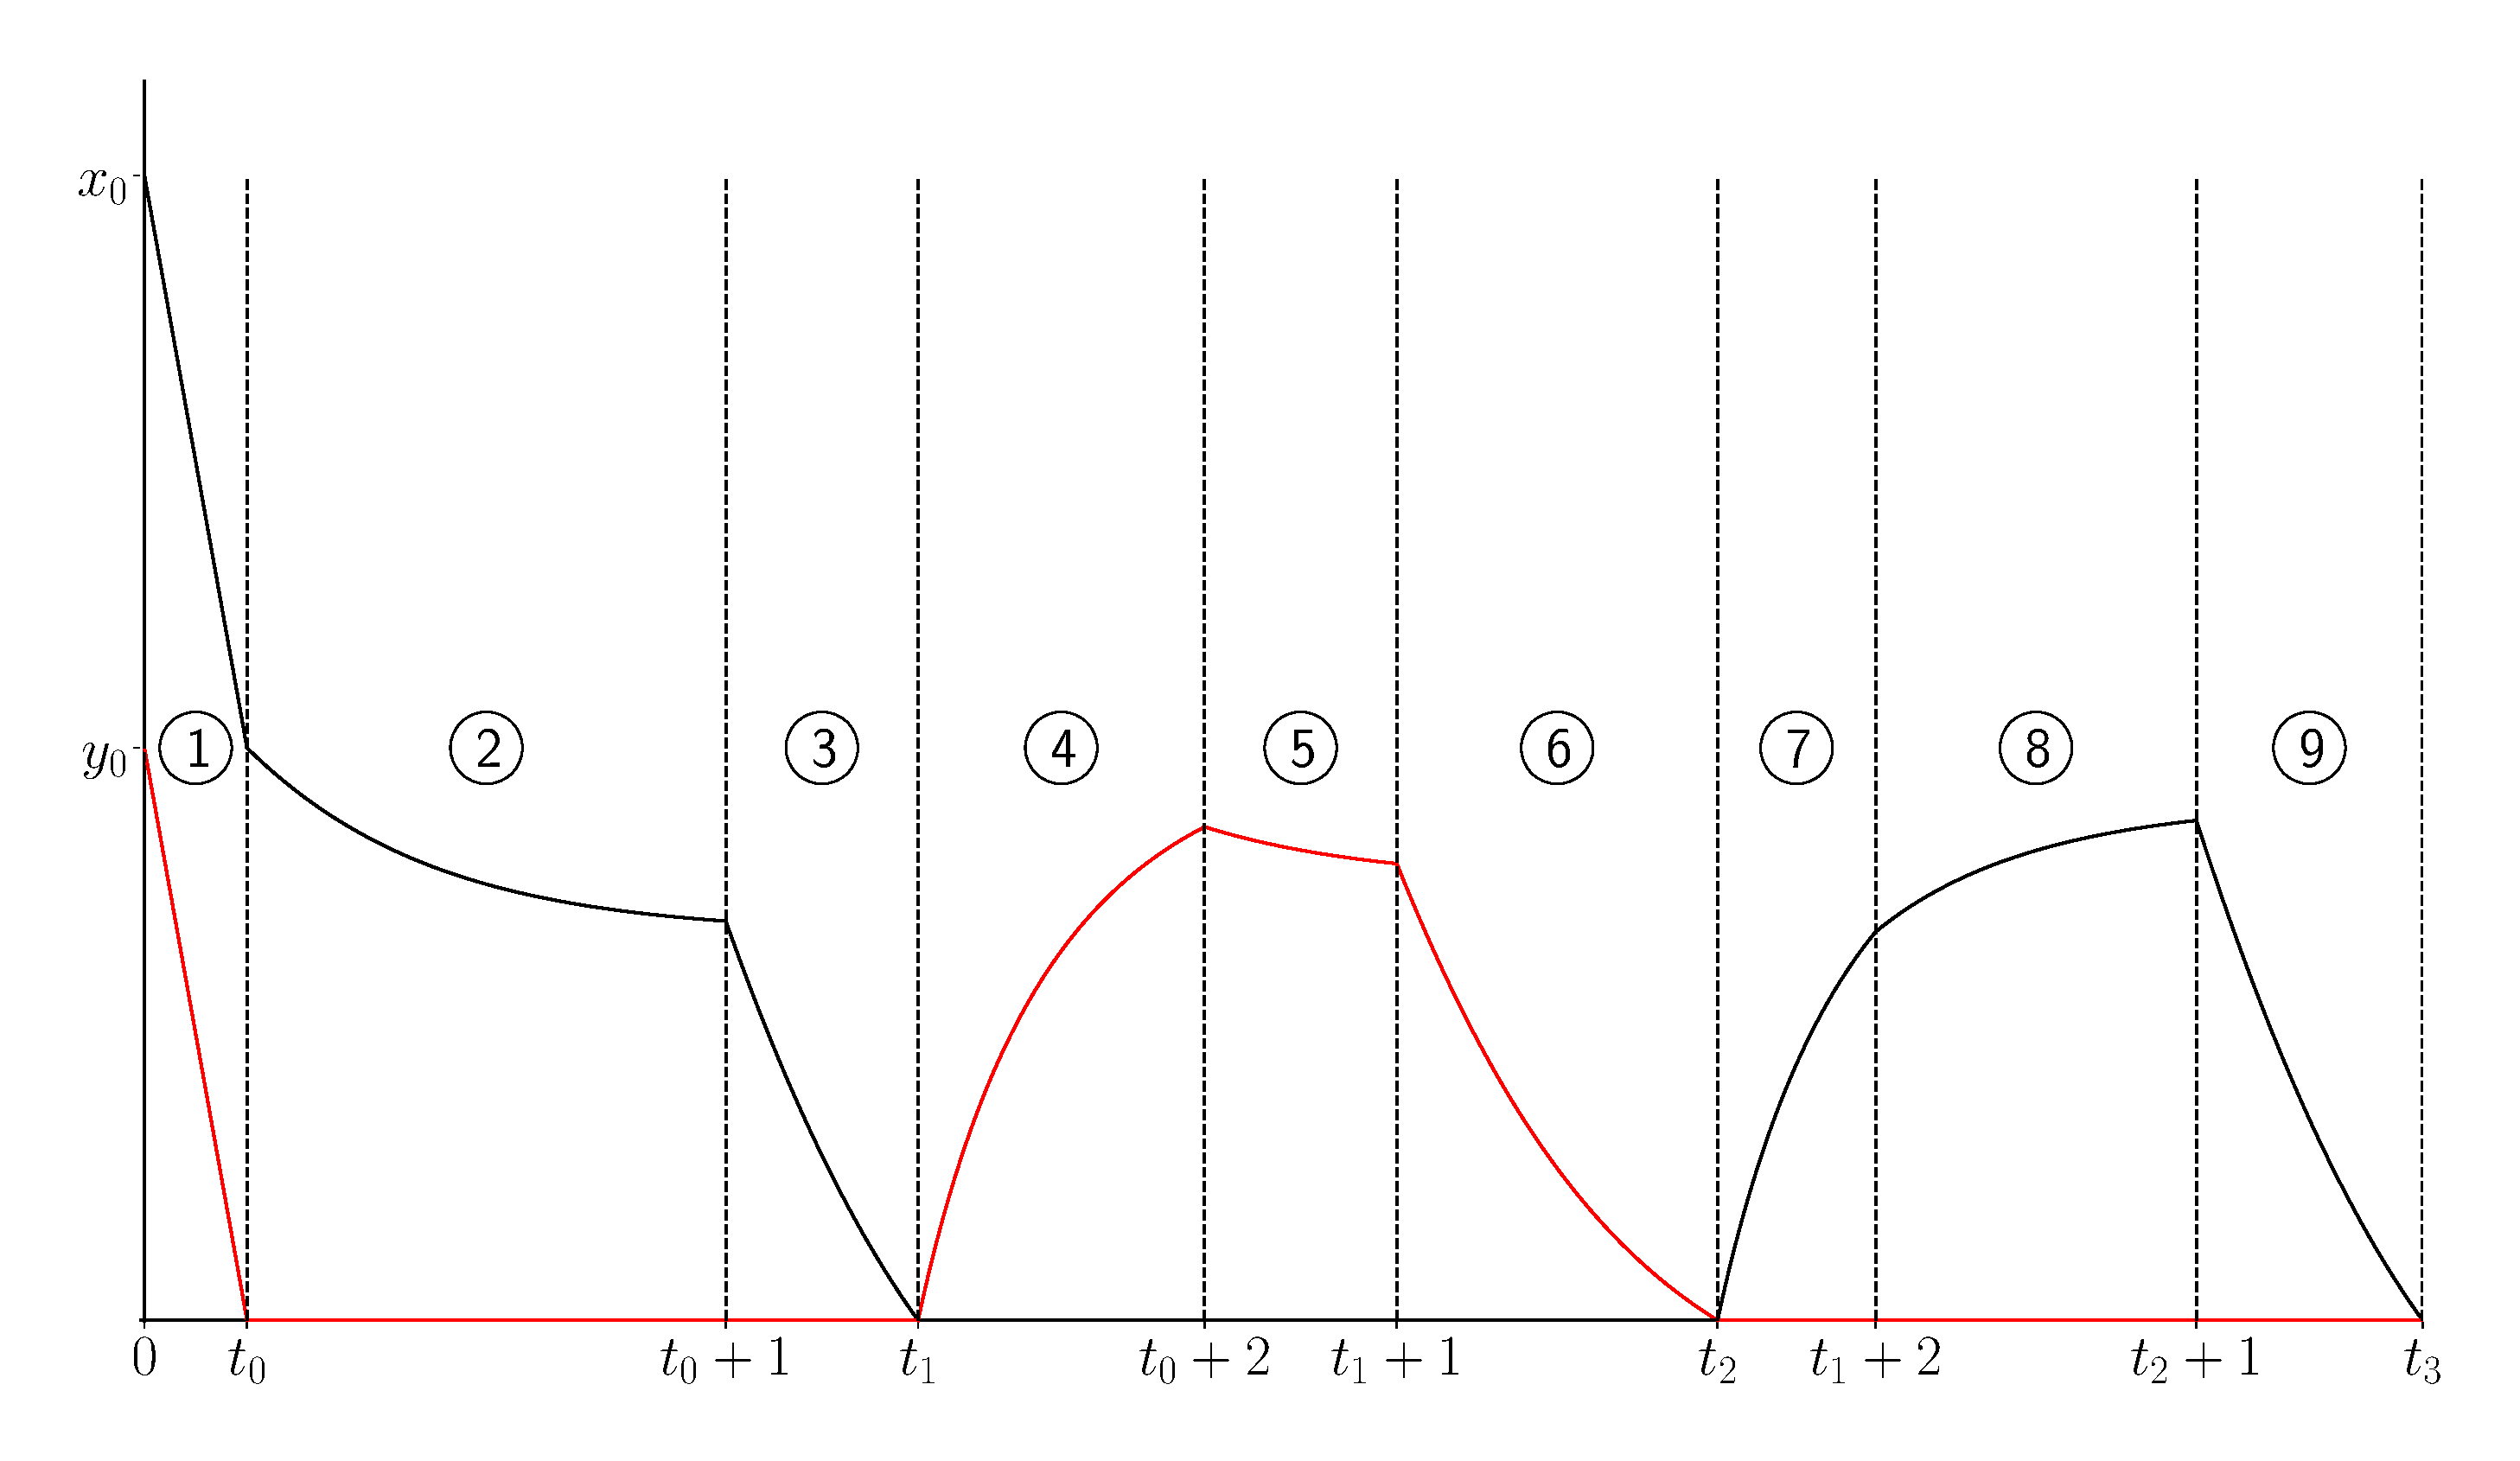
\includegraphics[width=0.9\linewidth]{cluster_step_by_step.eps}
\end{frame}


\begin{frame}
	\frametitle{Основная теорема}
	\textbf{Теорема 4.} При ограничениях на параметры из теоремы 3, существует периодическое обобщённое решение $x(t)$, $y(t)$ релейной системы, соответствующее шагам 4 -- 9 решения, описанного выше.
	
	\begin{center}
		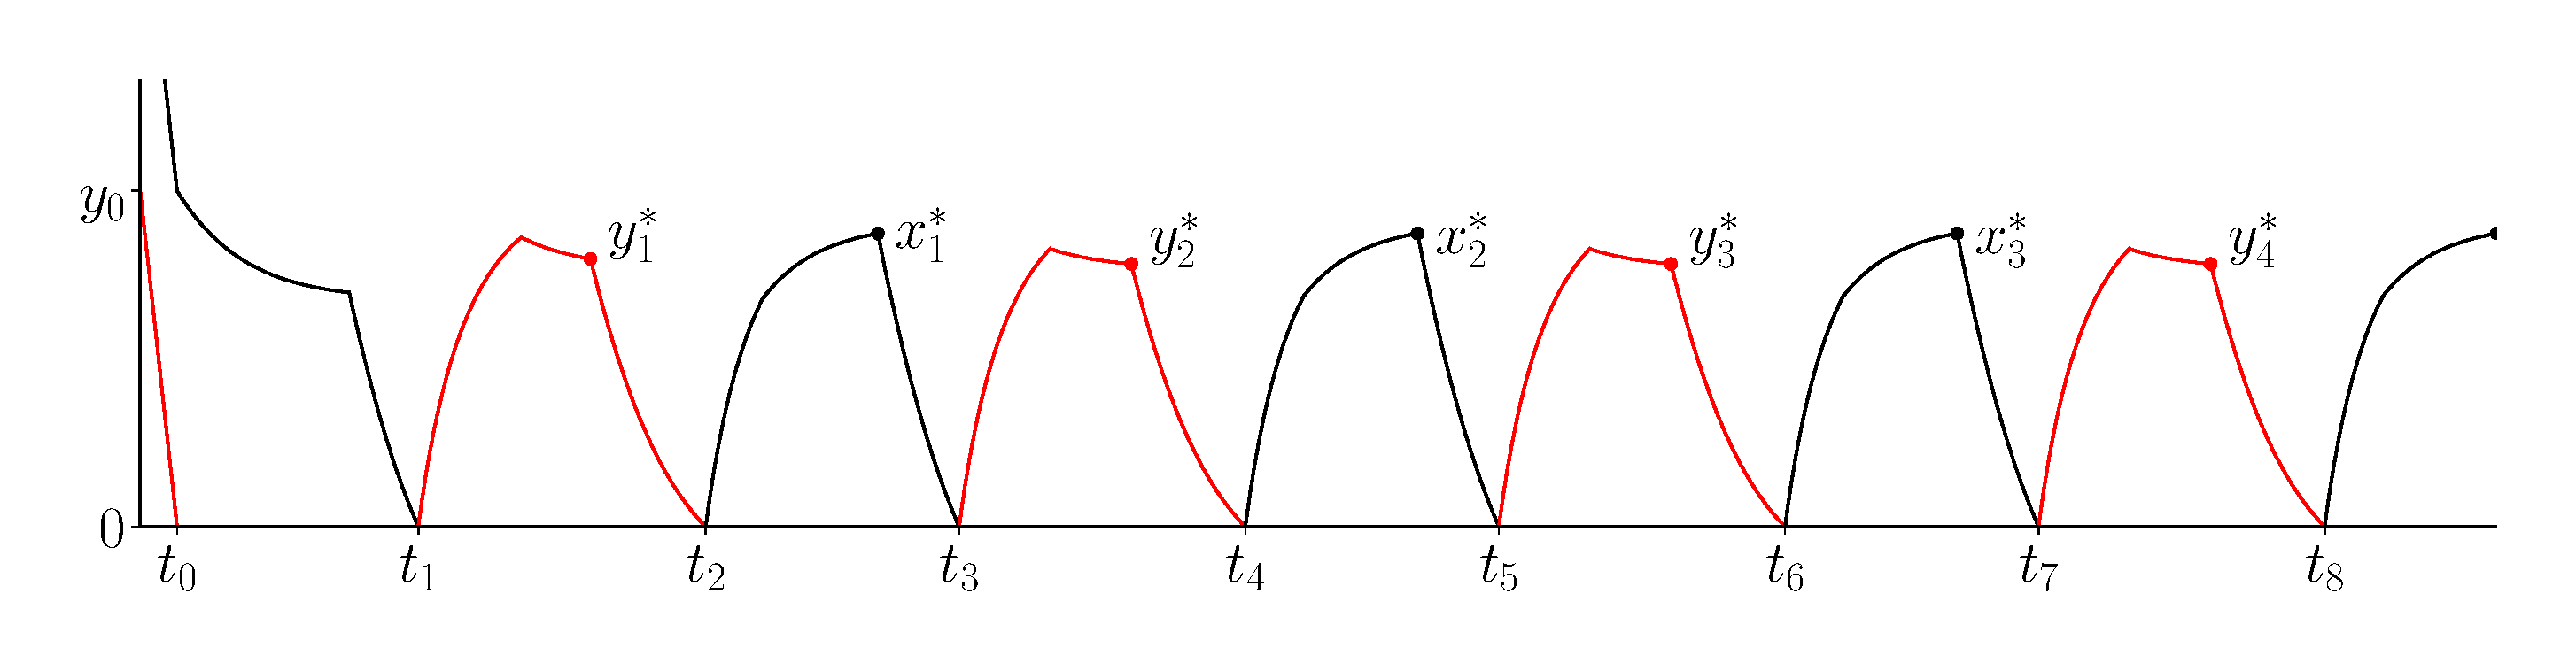
\includegraphics[width=\textwidth]{cluster_stars.eps}
	\end{center}
\end{frame}

\begin{frame}
	\frametitle{Численные результаты}
	\includegraphics[width=\linewidth]{cluster_solution_1.eps}
	
	\includegraphics[width=\linewidth]{cluster_solution_2.eps}
\end{frame}
